\documentclass[unicode,11pt,a4paper,oneside,numbers=endperiod,openany]{scrartcl}

\usepackage{amsmath}
\usepackage{amssymb}
\usepackage{multirow}
\usepackage{float}
\usepackage{graphicx}

\renewcommand{\thesubsection}{\arabic{subsection}}
\renewcommand{\arraystretch}{1.5} % Adjust the spacing between rows

\graphicspath{{./figures/}}


\input{assignment.sty}
\begin{document}


\setassignment
\setduedate{Wednesday, 22 November 2023, 11:59 PM}

\serieheader{Numerical Computing}{2023}
{\textbf{Student:} Jeferson Morales Mariciano\\}
{\textbf{Discussed with:} Leonardo Birindelli, Michele Dalle Rive, Martin Lettry, Sofia d'Atri}
{Bonus assignment}{}
\newline

\assignmentpolicy


\newpage

\section{Exercise: Inconsistent systems of equations [10 points]}
\label{sec:ex1}
Consider the following inconsistent systems of equations:

\begin{equation}
    A_1x = b_1,
    A_1 =
    \begin{bmatrix} 1 & 0 \\1 & 0 \\1 & 0 \\ \end{bmatrix}
    \in \mathbb{R}^{3 \times 2},
    b_1 =
    \begin{bmatrix} 5 \\ 2\\ 4 \\ \end{bmatrix}
\end{equation}

\begin{equation}
    A_2x = b_2,
    A_2 =
    \begin{bmatrix} 1 & 1 & 0 \\0 & 1 & 1 \\1 & 2 & 1 \\1 & 0 & 1 \\ \end{bmatrix}
    \in \mathbb{R}^{4 \times 3},
    b_2 =
    \begin{bmatrix} 2 \\ 2\\ 3\\ 4\\ \end{bmatrix}
\end{equation}

Find the least squares solution $x^*$ and compute Euclidean norm of the residual, SE, RMSE.

\subsection{}
\[
    A^{\top}A x^* = A^{\top}b
\]
\begin{equation*}
    \begin{aligned}
        A^{\top}A &
        =
        \begin{bmatrix} 1 & 1 & 1 \\ 0 & 0 & 0 \\ \end{bmatrix}
        \cdot
        \begin{bmatrix} 1 & 0 \\ 1 & 0 \\ 1 & 0 \\\end{bmatrix}
        =
        \begin{bmatrix} 3 & 0 \\ 0 & 0 \\ \end{bmatrix}
    \end{aligned}
\end{equation*}

\begin{equation*}
    \begin{aligned}
        A^{\top}b &
        =
        \begin{bmatrix} 1 & 1 & 1 \\ 0 & 0 & 0 \\ \end{bmatrix}
        \cdot
        \begin{bmatrix} 5 \\ 2 \\ 4\\ \end{bmatrix}
        =
        \begin{bmatrix} 11 \\ 0 \\ \end{bmatrix}
    \end{aligned}
\end{equation*}

\[
    \begin{bmatrix} 3 & 0 \\ 0 & 0 \\ \end{bmatrix} x^*
    =
    \begin{bmatrix} 11 \\ 0 \\ \end{bmatrix}
\]

\begin{equation*}
    \begin{cases} 3x_1 = 11 \\ 0x_2 = 0  \\ \end{cases}
    \rightarrow
    \begin{cases} x_1 = \frac{11}{3} \\ x_2 \in \mathbb{R} \\ \end{cases}
\end{equation*}

\[
    r
    = b - Ax^*
    = \begin{bmatrix} 5 \\ 2 \\ 4\\ \end{bmatrix}
    -
    \begin{bmatrix} 1 & 0 \\ 1 & 0 \\ 1 & 0 \\ \end{bmatrix}
    \begin{bmatrix} \frac{11}{3} \\ 0\\ \end{bmatrix}
    =
    \begin{bmatrix} 5 \\ 2 \\ 4\\ \end{bmatrix}
    -
    \frac{11}{3} \begin{bmatrix} 1 \\ 1\\ 1\\ \end{bmatrix}
    =
    \frac{1}{3} \begin{bmatrix} 4 \\ -5 \\ 1\\ \end{bmatrix}
\]
\[
    euclidean\_norm
    = ||r||_2 = \sqrt{\sum_{i=1}^{n}r_i^2}
    = \frac{\sqrt{42}}{3}
    \approx 2.1602
\]
\[
    SE
    = ||r||_2^2 = \sum_{i=1}^{n}r_i^2
    = \frac{42}{9}
    \approx 4.6665
\]
\[
    RMSE
    = \frac{euclidean\ norm}{\sqrt{\# equations}}
    = \frac{\frac{\sqrt{42}}{3}}{\sqrt{3}}
    = \frac{\sqrt{126}}{9}
    \approx 1.2472
\]

\subsection{}
\begin{equation*}
    \begin{aligned}
        A^{\top}A &
        =
        \begin{bmatrix} 1 & 0 & 1 & 1 \\ 1 & 1 & 2 & 0 \\ 0 & 1 & 1 & 1 \\ \end{bmatrix}
        \cdot
        \begin{bmatrix} 1 & 1 & 0 \\0 & 1 & 1 \\1 & 2 & 1 \\1 & 0 & 1 \\ \end{bmatrix}
        =
        \begin{bmatrix} 3 & 3 & 2 \\ 3 & 6 & 3 \\ 2 & 3 & 3 \\ \end{bmatrix}
    \end{aligned}
\end{equation*}

\begin{equation*}
    \begin{aligned}
        A^{\top}b &
        =
        \begin{bmatrix} 1 & 0 & 1 & 1 \\ 1 & 1 & 2 & 0 \\ 0 & 1 & 1 & 1 \\ \end{bmatrix}
        \cdot
        \begin{bmatrix} 2 \\ 2 \\ 3 \\ 4 \\ \end{bmatrix}
        =
        \begin{bmatrix} 9 \\ 10 \\ 9 \\ \end{bmatrix}
    \end{aligned}
\end{equation*}

\[
    \begin{bmatrix} 3 & 3 & 2 \\ 3 & 6 & 3 \\ 2 & 3 & 3 \\ \end{bmatrix}
    x^*
    =
    \begin{bmatrix} 9 \\ 10 \\ 9 \\ \end{bmatrix}
\]

\begin{equation*}
    \begin{cases}
        3 x_1 + 3 x_2 + 2 x_3 = 9  \\
        3 x_1 + 6 x_2 + 3 x_3 = 10 \\
        2 x_1 + 3 x_2 + 3 x_3 = 9  \\
    \end{cases}
\end{equation*}

\begin{equation*}
    E_{32} \Bigl( -\frac{1}{3} \Bigr) \cdot E_{21} \Bigl( -1 \Bigr) \cdot E_{31} \Big( -\frac{2}{3} \Bigl)
    \cdot
    \begin{bmatrix} 3 & 3 & 2 \\ 3 & 6 & 3 \\ 2 & 3 & 3 \\ \end{bmatrix}
\end{equation*}

\begin{equation*}
    \begin{cases}
        3 x_1 + 3 x_2 + 2 x_3 = 9     \\
        3 x_2 + x_3 = 1               \\
        \frac{4}{3} x_3 = \frac{8}{3} \\
    \end{cases}
    \rightarrow
    \begin{cases}
        x_1 = 2             \\
        x_2 = - \frac{1}{3} \\
        x_3 = 2             \\
    \end{cases}
\end{equation*}

\[
    r
    =
    \begin{bmatrix} 2 \\ 2 \\ 3 \\ 4 \\ \end{bmatrix}
    -
    \begin{bmatrix} 1 & 1 & 0 \\0 & 1 & 1 \\1 & 2 & 1 \\1 & 0 & 1 \\ \end{bmatrix}
    \cdot
    \begin{bmatrix} 2 \\ - \frac{1}{3} \\ 2 \\ \end{bmatrix}
    =
    \begin{bmatrix} 2 \\ 2 \\ 3 \\ 4 \\ \end{bmatrix}
    -
    \frac{1}{3} \begin{bmatrix} 5 \\ 5 \\ 10 \\ 12 \\ \end{bmatrix}
    =
    \frac{1}{3} \begin{bmatrix} 1 \\ 1 \\ -1 \\ 0 \\ \end{bmatrix}
\]
\[
    euclidean\_norm
    = \frac{\sqrt{3}}{3}
    \approx 0.5774
\]
\[
    SE
    = \frac{1}{3}
    \approx 0.3333
\]
\[
    RMSE
    = \frac{\frac{\sqrt{3}}{3}}{\sqrt{4}}
    = \frac{\sqrt{3}}{6}
    \approx 0.2887
\]


\section*{Exercise 2: Polynomials models for least squares [20 points]}

In this exercise, we consider two small datasets about the crude oil (\textit{crudeOil.txt})
and kerosene (\textit{kerosene.txt}) production by year in Europe in the period $1980-2012$.
By solving the following tasks, we will try to fit the data with different polynomial models
and determine the best one.\\

Source code of exercises are in \textit{./ex2} folder.

\subsection*{a}
The \textit{leastSquares.m} function is implemented and correctly returning the solution computed manually in
Exercise \ref{sec:ex1} when checked with \textit{ex2a.m} script.\\
Solution $x^*$, Euclidean norm of the residual, SE, RMSE are computed and printed in the console.

\subsection*{b}
Both crude oil and kerosene data during the period $1980-2011$ got their least square solution and metrics in
the script \textit{linearModel.m} using a linear model. \\
Table \ref{table:ex2} summarize x* and metrics for both datasets. \\
Plot \ref{fig:ex2-oil} refers to crude oil dataset case and Plot \ref{fig:ex2-kerosene} to kerosene dataset case.

\begin{figure}[H]
    \centering
    \caption{Crude oil dataset - linear model}
    \label{fig:ex2-oil}
    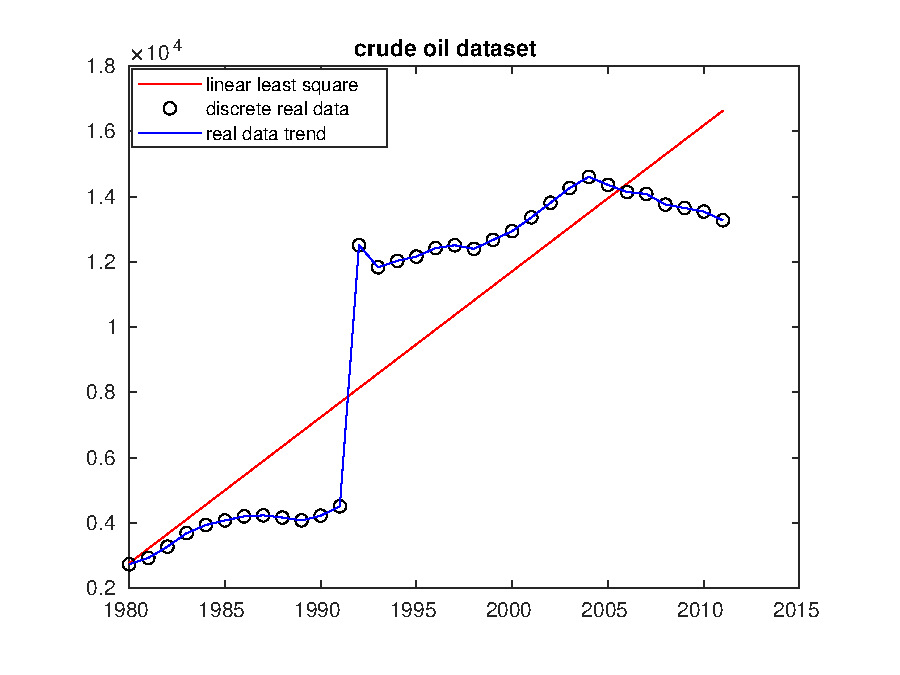
\includegraphics[width=0.8\textwidth]{ex2-oil.eps}
\end{figure}

\begin{figure}[H]
    \centering
    \caption{Kerosene dataset - linear model}
    \label{fig:ex2-kerosene}
    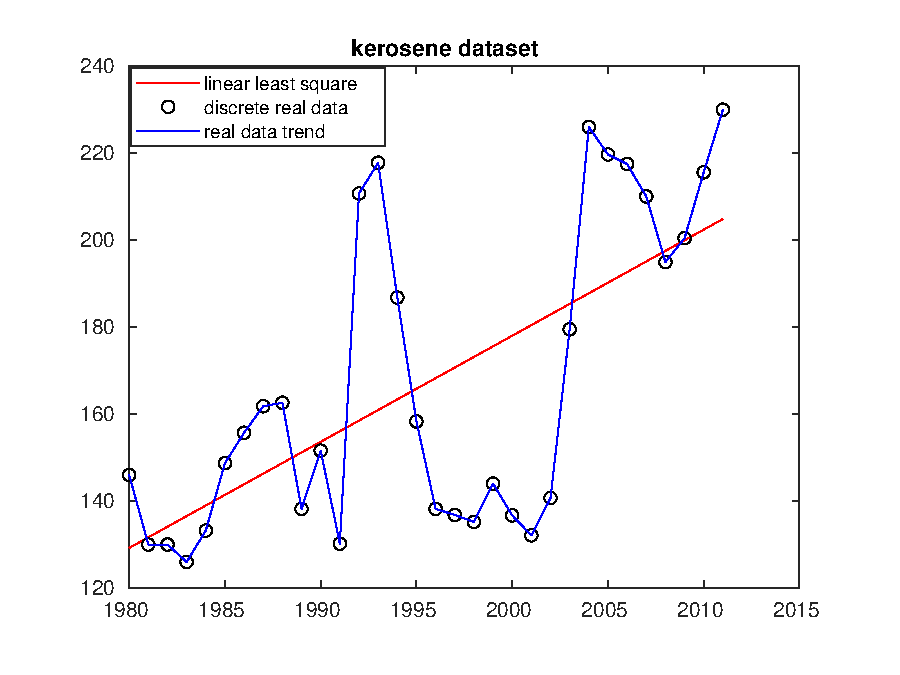
\includegraphics[width=0.8\textwidth]{ex2-kerosene.eps}
\end{figure}

\subsection*{c}
The same procedure of the previous task is repeated using a quadratic model in \textit{quadraticModel.m} script. \\
Table \ref{table:ex2c} summarize x* and metrics for both datasets. \\
Plot \ref{fig:ex2c-oil} refers to crude oil dataset case and Plot \ref{fig:ex2c-kerosene} to kerosene dataset case.

\begin{figure}[H]
    \centering
    \caption{Crude oil dataset - quadratic model}
    \label{fig:ex2c-oil}
    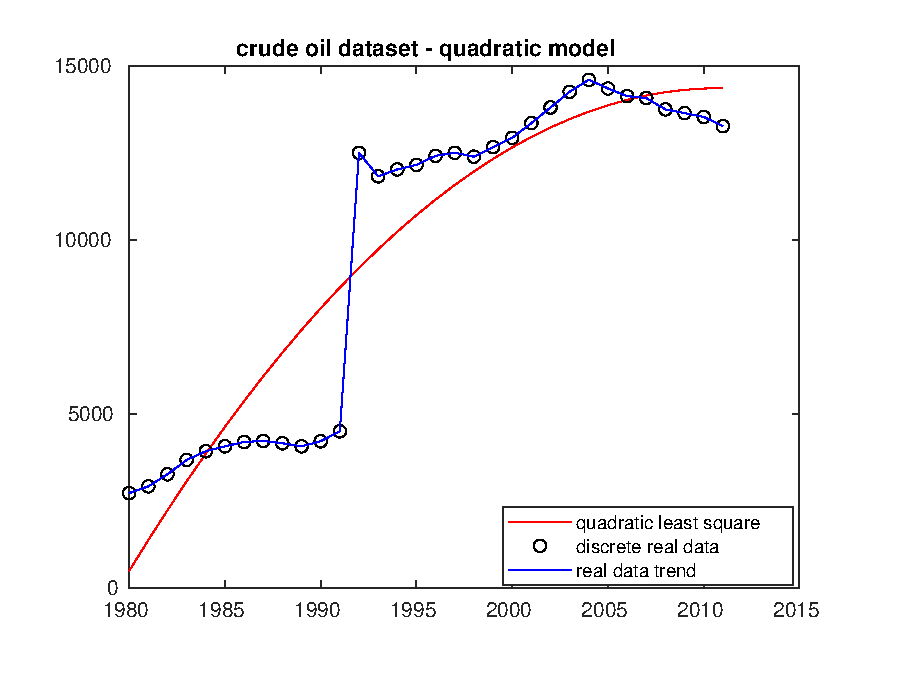
\includegraphics[width=0.8\textwidth]{ex2c-oil.eps}
\end{figure}

\begin{figure}[H]
    \centering
    \caption{Kerosene dataset - quadratic model}
    \label{fig:ex2c-kerosene}
    \includegraphics[width=0.8\textwidth]{ex2c-kerosene.eps}
\end{figure}

\subsection*{d}
The same procedure of the previous task is repeated using a cubic model in \textit{cubicModel.m} script. \\
Table \ref{table:ex2d} summarize x* and metrics for both datasets. \\
Plot \ref{fig:ex2d-oil} refers to crude oil dataset case and Plot \ref{fig:ex2d-kerosene} to kerosene dataset case.

\begin{figure}[H]
    \centering
    \caption{Crude oil dataset - cubic model}
    \label{fig:ex2d-oil}
    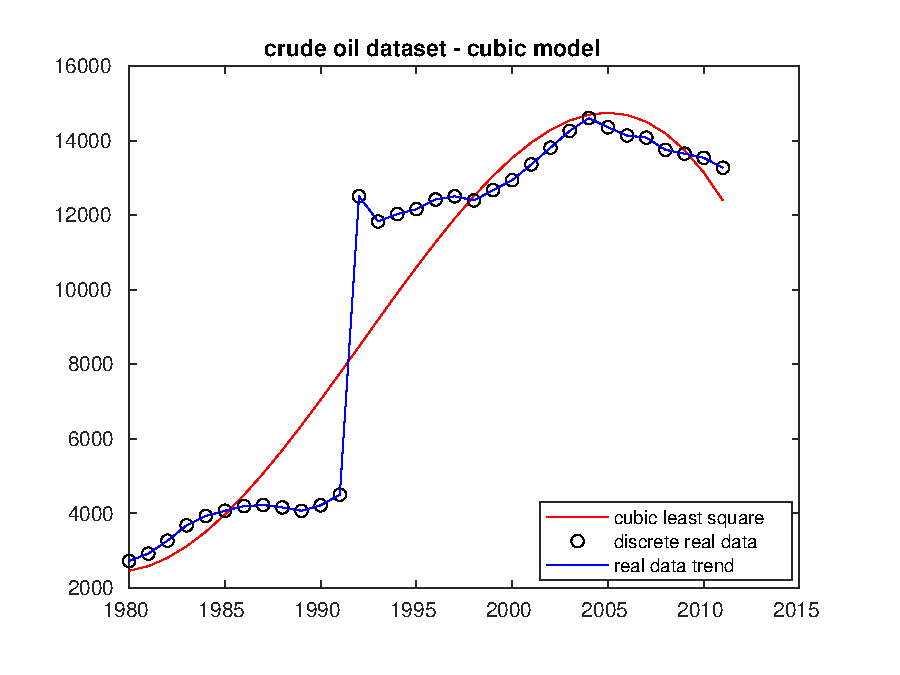
\includegraphics[width=0.8\textwidth]{ex2d-oil.eps}
\end{figure}

\begin{figure}[H]
    \centering
    \caption{Kerosene dataset - cubic model}
    \label{fig:ex2d-kerosene}
    \includegraphics[width=0.8\textwidth]{ex2d-kerosene.eps}
\end{figure}

\subsection*{e}
\subsubsection*{
    Compare the linear, quadratic and cubic models on the basis of the quality metrics computed above, by creating
    a table containing the results for the two models. Which one of the three models would you pick for the crude
    oil data? And for the kerosene?}

\begin{table}[H]
    \centering
    \caption{Crude oil and kerosene dataset metrics using linear model}
    \label{table:ex2}
    \begin{tabular}{||l l l l l||}
        \hline
        \slash   & $x^*$                                                               & euclidean norm & SE         & RMSE       \\
        \hline\hline
        oil      & $(1.0e+05) \cdot \begin{bmatrix} -8.8339 & 0.0045 \\ \end{bmatrix}$ & 1.1471e+04     & 1.3159e+08 & 2.0278e+03 \\
        kerosene & $(1.0e+03) \cdot \begin{bmatrix} -4.7013 & 0.0024 \\ \end{bmatrix}$ & 151.0222       & 2.2808e+04 & 26.6972    \\
        \hline
    \end{tabular}
\end{table}

\begin{table}[H]
    \centering
    \caption{Crude oil and kerosene dataset metrics using quadratic model}
    \label{table:ex2c}
    \begin{tabular}{||l l l l l||}
        \hline
        \slash   & $x^*$                                                                         & euclidean norm & SE         & RMSE       \\
        \hline\hline
        oil      & $(1.0e+07) \cdot \begin{bmatrix} -5.9181 & 0.0059 & -0.0000 \\ \end{bmatrix}$ & 9.5826e+03     & 9.1827e+07 & 1.6940e+03 \\
        kerosene & $(1.0e+05) \cdot \begin{bmatrix} 3.7596 & -0.0038 & 0.0000 \\ \end{bmatrix}$  & 145.3013       & 2.1112e+04 & 25.6859    \\
        \hline
    \end{tabular}
\end{table}

\begin{table}[H]
    \centering
    \caption{Crude oil and kerosene dataset metrics using cubic model}
    \label{table:ex2d}
    \begin{tabular}{||l l l l l||}
        \hline
        \slash   & $x^*$                                                                                  & euclidean norm & SE         & RMSE       \\
        \hline\hline
        oil      & $(1.0e+10) \cdot \begin{bmatrix} 1.1560 & -0.0017 & 0.0000 & -0.0000 \\ \end{bmatrix}$ & 7.9179e+03     & 6.2692e+07 & 1.3997e+03 \\
        kerosene & $(1.0e+07) \cdot \begin{bmatrix} -9.4357 & 0.0142 & -0.0000 & 0.0000 \\ \end{bmatrix}$ & 138.4756       & 1.9175e+04 & 24.4793    \\
        \hline
    \end{tabular}
\end{table}

The best model for both crude oil and kerosene datasets is the cubic model,
because it has the lowest lowest metrics overall: euclidean norm, SE and RMSE. \\

Such result can be due the rigidness of the linear model, which is not able to fit the data well,
and the flexibility and adaptability of the cubic model which is the best to describe the dynamic evolution of the datasets.

\subsubsection*{
    Provide an estimate of the crude oil and kerosene production in $2012$ by using
    the three models and compare the values obtained with the real values reported in the data source. Comment on
    your results.}

\begin{table}[H]
    \centering
    \caption{Estimate of 2012 for crude oil and kerosene dataset}
    \label{table:ex2d}
    \begin{tabular}{||l l l l l||}
        \hline
        dataset  & real sample & linear    & quadratic & cubic     \\
        \hline\hline
        oil      & 13,111.91   & 17,081.92 & 14,344.11 & 11,472.59 \\
        kerosene & 267.89      & 207.28    & 225.16    & 248.57    \\
        \hline
    \end{tabular}
\end{table}

Analyzing the data, it is seen clearly that for kerosene dataset the cubic model is the best one to fit the data
than the results returned from the rest, which are really far from the real sample.
Such behavior can be explained by the fact that the kerosene dataset is the most dynamic and scattered one.\\
For crude oil, the quadratic model is the one that best fit the real sample of $2012$, but indeed the cubic model
is also very accurate and in general, the models are not so far from the real sample.\\

\section*{Exercise 3: Analysis of periodic data [20 points]}

In this exercise, we consider the following dataset about the mean temperature in Switzerland
between January 1864 and March 2021 included in the (\textit{temperature.txt}) file.
Aim is to capture the periodic behaviour of the data by using periodic models.\\

Source code of exercises are in \textit{./ex3} folder.

\subsection*{a}

Script file \textit{periodicA.m} contains the solution.

\subsubsection*{I}

\begin{figure}[H]
    \centering
    \caption{Switzerland Jan 1960 to Jan 1963 mean temperature}
    \label{fig:ex3a-i}
    \includegraphics[width=0.8\textwidth]{ex3a-i.eps}
\end{figure}

\subsubsection*{II}

\begin{figure}[H]
    \centering
    \caption{Switzerland Jan 1960 to Jan 1970 mean temperature}
    \label{fig:ex3a-ii}
    \includegraphics[width=\textwidth]{ex3a-ii.eps}
\end{figure}

\subsection*{b}

Script file \textit{periodicB.m} contains the solution.

\subsubsection*{I}

\begin{figure}[H]
    \centering
    \caption{Switzerland Jan 1960 to Jan 1963 mean temperature}
    \label{fig:ex3b-i}
    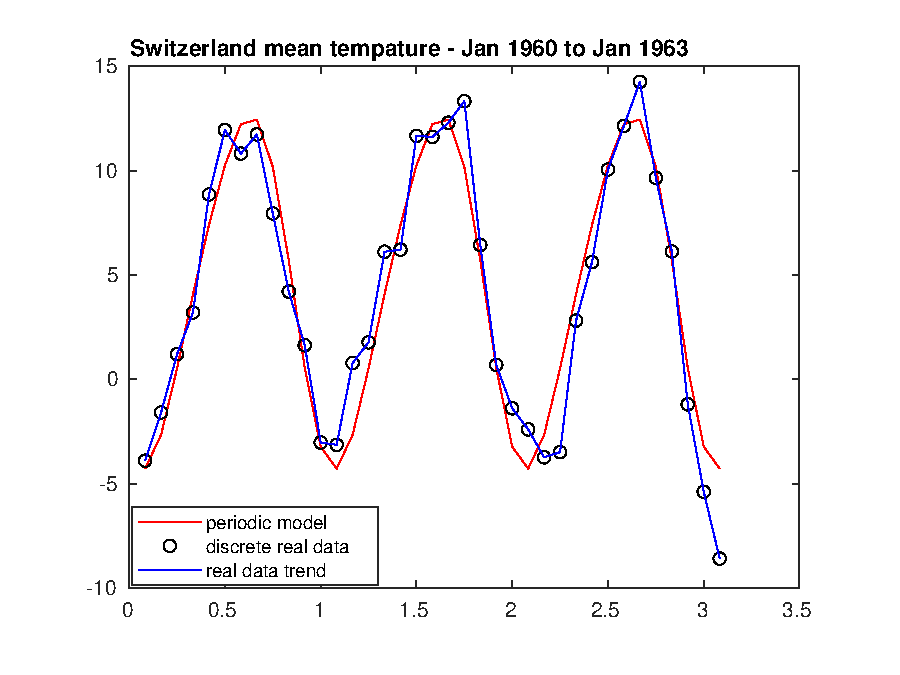
\includegraphics[width=0.8\textwidth]{ex3b-i.eps}
\end{figure}

\subsubsection*{II}

\begin{figure}[H]
    \centering
    \caption{Switzerland Jan 1960 to Jan 1970 mean temperature}
    \label{fig:ex3b-ii}
    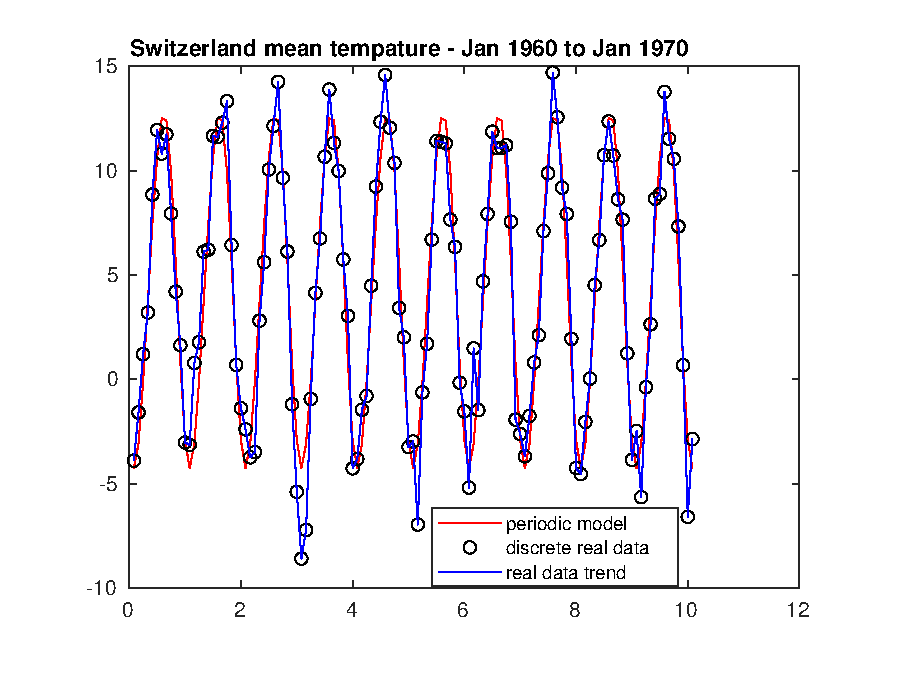
\includegraphics[width=\textwidth]{ex3b-ii.eps}
\end{figure}

\subsection*{c}

\begin{table}[H]
    \centering
    \caption{Metrics of the first periodic model}
    \label{table:ex3c-first}
    \begin{tabular}{||l l l l l||}
        \hline
        datasets            & $x^*$                                                         & euclidean norm & SE       & RMSE   \\
        \hline\hline
        Jan 1960 - Jan 1963 & $\begin{bmatrix} 4.4166 & -6.7605 & -4.8397\\ \end{bmatrix}$  & 11.2223        & 125.9405 & 1.8449 \\
        Jan 1960 - Jan 1963 & $\begin{bmatrix} 4.3816 & -6.7751 & -5.0419 \\ \end{bmatrix}$ & 18.0385        & 325.3890 & 1.6399 \\
        \hline
    \end{tabular}
\end{table}

\begin{table}[H]
    \centering
    \caption{Metrics of the second periodic model}
    \label{table:ex3c-second}
    \begin{tabular}{||l l l l l||}
        \hline
        datasets            & $x^*$                                                                   & euclidean norm & SE       & RMSE   \\
        \hline\hline
        Jan 1960 - Jan 1963 & $\begin{bmatrix}  4.4284 & -6.7401 & -4.8279 & -0.9191\\ \end{bmatrix}$ & 10.5138        & 110.5400 & 1.7285 \\
        Jan 1960 - Jan 1963 & $\begin{bmatrix} 4.3838 & -6.7713 & -5.0397 & -0.5321 \\ \end{bmatrix}$ & 17.5594        & 308.3312 & 1.5963 \\
        \hline
    \end{tabular}
\end{table}

Given the following data, it is seen that the second periodic model is the best one to fit the data,
since the metrics are lower than the first one.\\
The difference is not by magnitudes of order, but it is still significant.\\
The x coordinates for plotting the data are phased in 12 (twelves) to follow the periodicity of the data modelling years.\\
Hence, adding more terms to the model was beneficial to fit the data better, the second model is preferred over the first one.
Model results are satisfactory, but not perfect, since the data is not perfectly periodic.\\
A way to improve the model is to add more terms to the model, but the data among the phases are scattered and it
could be that in the future the more years we analyze, the more the phase goes out our model due to \textbf{climate change},
which will also need to be taken into account. \\

\section*{Exercise 4: Data linearization and Levenberg-Marquardt method for the exponential model [20 points]}

Source code of exercises are in \textit{./ex4} folder.

The file \textit{nuclear.txt} contains the data on the nuclear electric power consumption by year in China in the period
$1999-2006$. We consider the power law model:
\[
    y_i = \alpha_1 x_i^{\alpha_2}
\]

\subsection*{a}
Find the least squares best fit by using data linearization and compute the RMSE both of the log-linearized
model and of the original exponential model. Include in your report all the computations and the necessary
steps, as explained in the slides of the tutorial.\\

Using data linearization of the power law model we obtain the following least square best fit:
\[
    \alpha^* = \begin{bmatrix} 10.7026 & 0.7549 \\ \end{bmatrix}
\]

\begin{table}[H]
    \centering
    \caption{RMSE of models}
    \label{table:ex4a}
    \begin{tabular}{||l l||}
        \hline
        models               & RMSE    \\
        \hline\hline
        log linearized model & 0.20423 \\
        power law model      & 4.8141  \\
        \hline
    \end{tabular}
\end{table}

\subsection*{b}
Write a function levenbergMarquardt() in which you implement the Levenberg-Marquardt algorithm for
solving nonlinear least squares problems.
Following again the slides of the tutorial, show how you can formulate
the problem in order to solve it with Levenberg-Marquardt method and compute analytically all the necessary
quantities.
Finally, write a script ex4b.m in which you use the function levenbergMarquardt() to fit
the data points and compute the RMSE.\\

\[
    \alpha^* = \begin{bmatrix} 8.2502 & 0.9299 \\ \end{bmatrix}
\]

\subsection*{c}

\begin{figure}[H]
    \centering
    \caption{nuclear dataset - power law model}
    \label{fig:ex4c}
    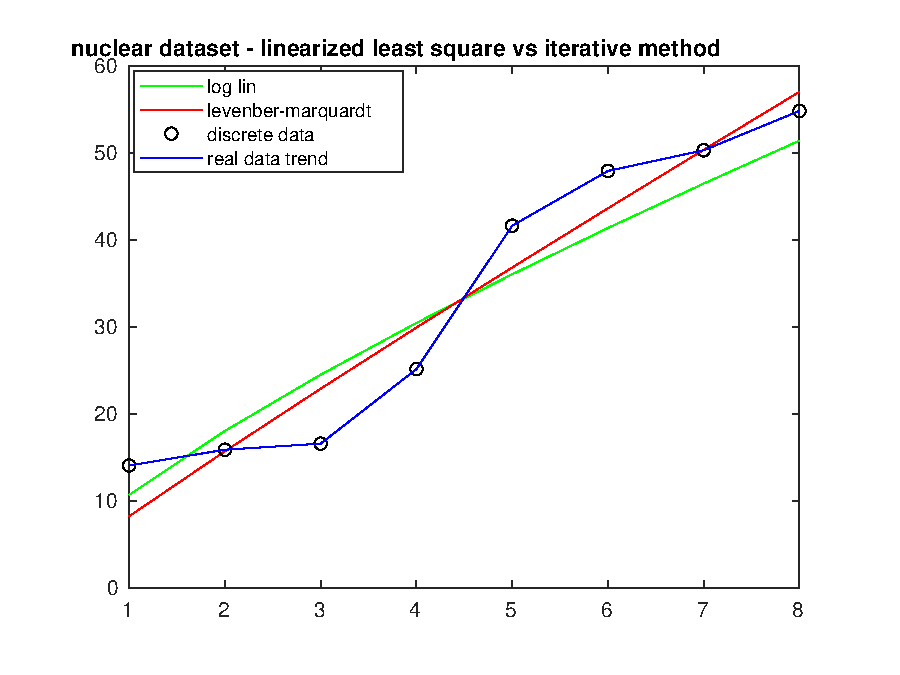
\includegraphics[width=\textwidth]{ex4c.eps}
\end{figure}

Given the following metrics:

%\begin{table}[H]
%    \centering
%    \caption{Metrics of nuclear dataset}
%    \label{table:ex4c}
%    \begin{tabular}{||l l l l||}
%        \hline
%        datasets                       & euclidean norm & SE       & RMSE   \\
%        \hline\hline
%        log linearized power law model & 0.5777         & 0.3337   & 0.2042 \\
%        levenberg-Marquardt            & 11.9675        & 143.2204 & 4.2311 \\
%        \hline
%    \end{tabular}
%\end{table}

The Levenberg - Marquardt is preferred since it shows slightly lower metrics than means that the model is better to fit the data.\\
The plot above shows a better slope orientation for the levenberg Marquardt model than the log linearized power law model.\\

\section*{Exercise 5: Tikhonov regularization [15 points]}

\subsection*{a}

Given the Tikhonov regularization denominated as $f(x)$:
\[
    f(x) = \min_{x} ||Ax - b||_2^2 + \alpha ||x||_2^2
\]
Find its gradient:
\[
    \nabla f(x) = 2A^{\top}Ax - 2A^{\top}b + 2\alpha x
\]
x is defined as:
\[
    x = (A^{\top}A + \alpha I)^{-1}A^{\top}b
\]
Where $I$ is the identity matrix.\\
This solution equals the minimum of the Tikhonov regularization, when the derivative is set to 0.\\
The additional regularization term $\alpha ||x||_2^2$ encourages small $x_i$ values to avoid overfitting.

\subsection*{b}
Produce also two figures
in which you plot: the condition number of H (use cond() in Matlab) against n; the norm of the error
$||x_{exact} - x||_2$ against $n$

\begin{figure}[H]
    \centering
    \caption{Plot using Tikhonov regularization}
    \label{fig:ex5b}
    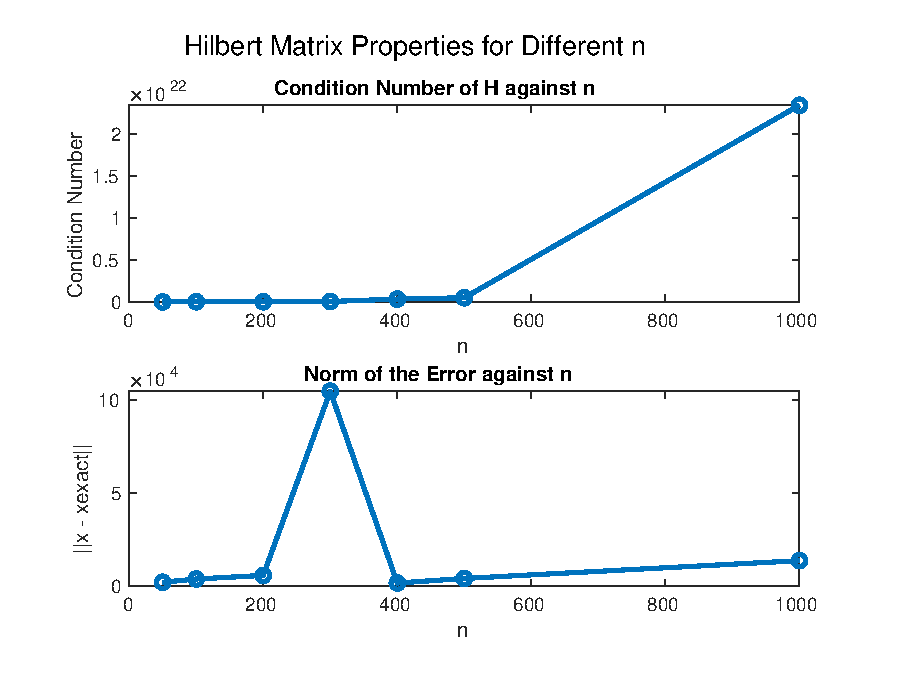
\includegraphics[width=\textwidth]{ex5b.eps}
\end{figure}

\subsection*{c}
To visualize the results, produce two figures in which you plot:
the norm of the error $||x_{exact} - x_{reg}||_2$ against the values of $\alpha$; $||H_x - b||_2 against ||x||_2$
for the different values of $\alpha$. Comment your results

\begin{figure}[H]
    \centering
    \caption{Plot using Tikhonov reagularization with different $\alpha$ values}
    \label{fig:ex5c}
    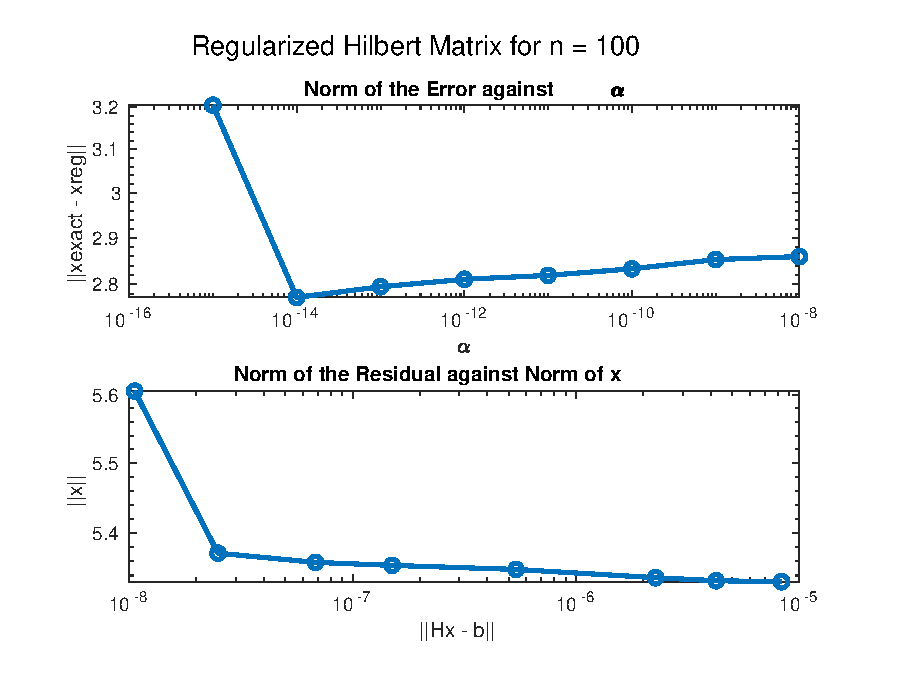
\includegraphics[width=\textwidth]{ex5c.eps}
\end{figure}

\end{document}
